% Chapter Template

\chapter{Results} % Main chapter title

\label{Chapter4} % Change X to a consecutive number; for referencing this chapter elsewhere, use \ref{ChapterX}

%----------------------------------------------------------------------------------------
%	SECTION 1
%----------------------------------------------------------------------------------------
\section{Finding The Correlated Photons}

SPDC nocolinear type II
\begin{figure}[h!]
\centering
{  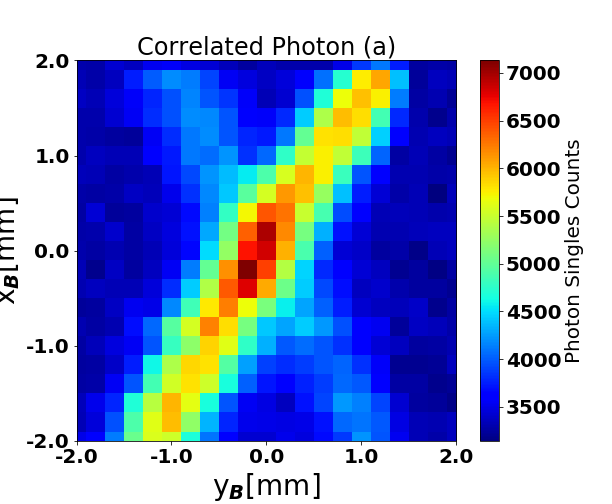
\includegraphics[width=0.45\textwidth]{Figures/correlatedPhotonSpot1.png} }
{  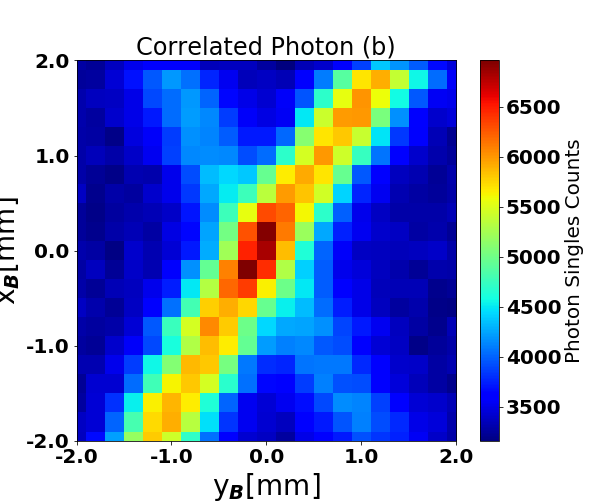
\includegraphics[width=0.45\textwidth]{Figures/correlatedPhotonSpot2.png} }
\caption{We are moving the translational translational stage, to locate the spot where the correlated photon are, for this try me moved the $y$ direction}
 \label{fig:correlatedPhotonSpot}
\end{figure}


\section{Experimental Correlations }

Info taken before me 
%-----------------------------------
%	SUBSECTION 1
%-----------------------------------
\subsection{$w_p = ?$}

\section{Mask Alignment}
We want that most of the correlated photon hits the mask 

\begin{figure}[h!]
\centering
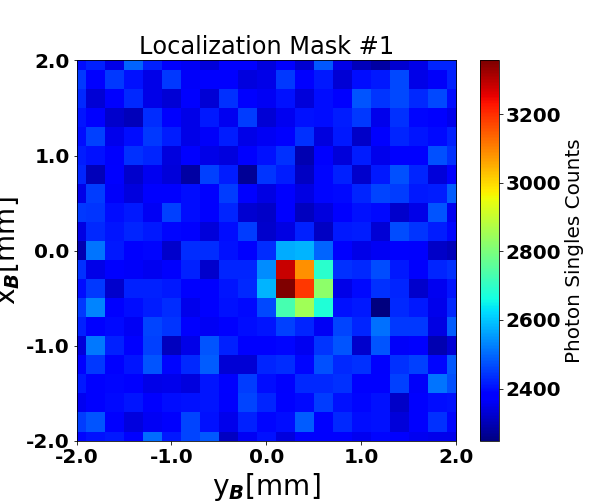
\includegraphics[width=0.6\textwidth]{Figures/localizationSq.png} 
\caption{Localization of the mask with an square}
\label{fig:localizationSq}
\end{figure}

changing to the mask with an L

\begin{figure}[h!]
\centering
{  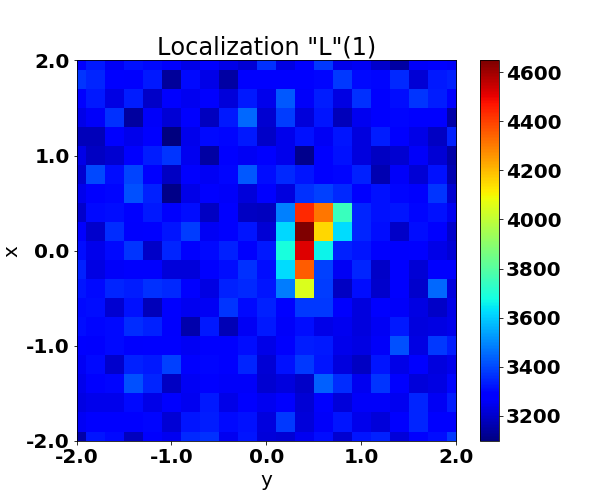
\includegraphics[width=0.45\textwidth]{Figures/localizationL1.png} }
{  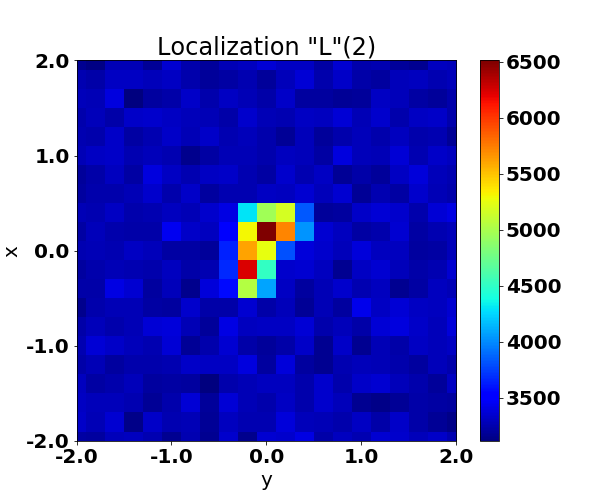
\includegraphics[width=0.45\textwidth]{Figures/localizationL2.png} }
\caption{Moving the L Mask in order to put it in the most central spot}
 \label{fig:localizationL}
\end{figure}
Long Exposure
\begin{figure}[h!]
\centering
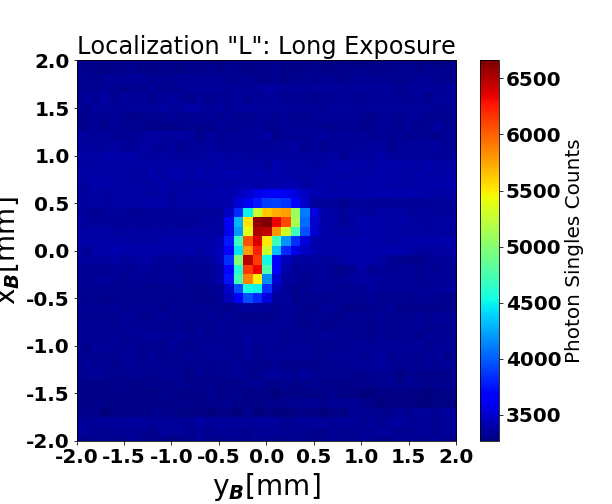
\includegraphics[width=0.6\textwidth]{Figures/localizationLLong.png} 
\caption{Long exposure of the definitive localization of the mask, in this try we leave the 
detector in each place for 30 seconds, we also make the steps of the detector smaller, $0.1mm$}
\label{fig:localizationDef}
\end{figure}

\section{Two-Photon Images}


\subsection{mask1}
\begin{figure}[h!]
\centering
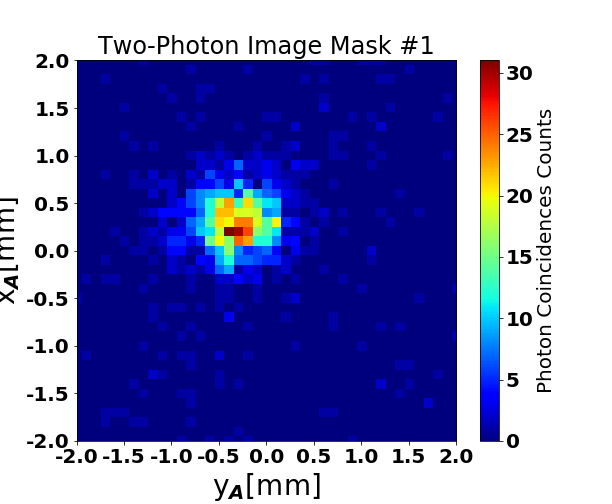
\includegraphics[width=0.6\textwidth]{Figures/two-photonImageSq.png} 
\caption{Localization of the mask with an square}
\label{fig:localizationSq}
\end{figure}

\subsection{mask2}
\subsection{mask3}
